%!TEX root = ../fbi.tex

\section{Conclusion and Discussion}

\appendix

\section{Determining the edge action of the symmetry using MPS}
\label{Appendix:MPS}

We can use the formalism of MPS to assign an action
of the symmetry on the Schmidt states, and in particular for the charge and 
translation on-site symmetries the Schmidt states can be simultaneously assigned
charge and translation quantum numbers. This method of discovering the symmetry 
action will reproduce the action discussed in \ref{sec:ES} and quantum numbers used
in the spectra plots shown in Fig.~\ref{fig:ESL910}.
  
Let's discuss this formalism briefly. In addition,
we will discuss a generalization of this method that allows us to numerically
determine the symmetry action of inversion symmetry on the Schmidt states,
as in Section~\ref{sec:symmetry}. 
Both of these discussions follow Ref.~\onlinecite{pollmann2010}.

These discussions start by finding tensors $\Gamma, \Lambda$ representing the 
so-called canonical form of the MPS, as
originally detailed in \cite{perezgarcia2008}. This canonical form provides the Schmidt
decomposition at each site in the lattice.
\beq
\ket{\psi} = \sum\limits_{\{p_i\}} \ldots \Lambda \Gamma_{p_0} \Lambda \Gamma_{p_1} \Lambda \Gamma_{p_2} \Lambda \ldots \ket{... p_0 p_1 p_2 ...}.
\eeq
As a reminder, each physical leg represents all $2W$ physical sites on a cylinder slice,
and each virtual leg represents all virtual indices that connect cylinder slices.
The change of basis to canonical form generally mixes the Hilbert spaces from these
virtual legs, so the resulting basis won't be local around the circumference
of the cylinder.

Each on-site symmetry of the wavefunction $U_g = \otimes_i u^i_g$, with $U_g
\ket{\psi} = e^{i \Theta_g} \ket{\psi}$ is assigned an operator $V_g$ that
acts on the virtual leg of the MPS, that satisfies the equation
\begin{center}
\beq
\label{eq:onsitesym}
\eeq
\vskip-5em
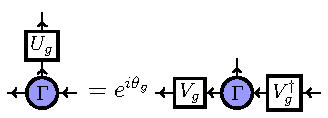
\includegraphics[width=0.6\columnwidth]{group_sym.pdf}.
\end{center}
This equation can be rewritten and solved as an eigenvector problem;
for an MPS with a nondegenerate largest transfer matrix eigenvalue,
this equation is guaranteed have a unique solution where the eigenvalue $e^{i \theta_g}$
is the largest eigenvalue of the eigenvector problem.

The solutions $V_g$ have two important properties: they are only defined up to a phase,
and they are guaranteed to commute with the diagonal matrix $\Lambda$ of Schmidt weights.  

Due to the first property, these operators are not guaranteed to form a linear
representation of the group of on-site symmetries, but in general could make
up a projective representation, satisfying
$$V_g V_h = e^{i \omega(g, h)} V_{gh}.$$ 
It is not always possible to absorb these phases into the definitions of the $V_g$.
Furthermore, the phases $\omega(g, h)$ can be classified into distinct group cohomology classes
$H^2(G, U(1))$ which cannot be connected to each other without breaking the symmetry.

The classification of projective representations for the on-site symmetry group $U(1) \times \mathbb{Z}_W$ representing charge and translation around the cylinder is trivial. Thus, the edge
symmetry can be taken to act linearly, and all Schmidt states can be simultaneously assigned 
charge and momentum eigenvalues. 

The second property guarantees that the $V_g$ only mixes exactly degenerate Schmidt states.
The action of $V_g$ must have the same phases $\omega(g, h)$ on each degenerate block of Schmidt states, so the projective representation can be nontrivial on any block only if every Schmidt state throughout the entire spectrum is degenerate. The degeneracy will be protected by the symmetry if and only if the $V_g$ form a nontrivial projective representation. 

Thus, this 1D SPT analysis can only potentially give an interesting answer for the odd $W$ states of the HFBI, where this exact degeneracy is seen throughout the spectrum. Nonetheless, we find there are no on-site symmetries of the wavefunction that can be used to explain the degenerate
entanglement spectrum of the odd $W$ HFBI states. Instead we must use an inversion symmetry. 

The MPS analysis of inversion symmetry starts similarly, but instead the tensor $\Gamma$ is 
transposed in the canonical basis. We will consider in general any symmetry of the wavefunction
that swaps the left and right half of the cylinder. 

\begin{center}
\beq
\label{eq:onsitesym}
\eeq
\vskip-5em
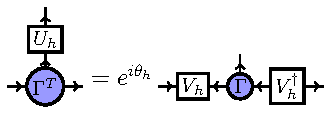
\includegraphics[width=0.6\columnwidth]{inv_sym.pdf}.
\end{center}

%In general, the $V_g$ do not have to form a linear representation of the
%group, but could instead be a projective representation. This can be explained
%in the MPS language as follows: if instead the blocks are connected together
%with different boundary conditions, as in Figure \ref{fig:mps_boundary}, we
%discover that $U_g$ transforms $\ket{\psi}$ to a similar state with
%transformed boundary conditions, $B \rightarrow V_g^{\dagger} B V_g$. This
%action on $B$, one can show, is a group representation.

%For open ends - if $B$ factors into left and right parts, $B =
%\vket{b}\vbra{b}$ - the action of the symmetry on the boundary can also be
%factored, $\vket{b} \rightarrow V_g \vket{b}$. This action does not have to be
%a group representation, but can fail up phases $V_g V_h = e^{i \omega(g, h)}
%V_{gh}$.

%\begin{figure}[htbc]
%    \centering
%    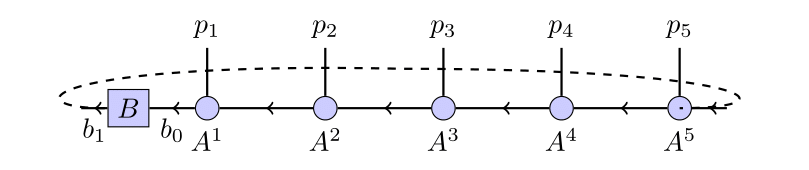
\includegraphics[width=\columnwidth]{mpsbc.png}
%    \caption{Matrix Product State with arbitrary boundary conditions}
%    \label{fig:mps_boundary}
%\end{figure}

%This symmetry action is determined on the Schmidt basis, but we can also
%change back to the basis determined by the virtual legs of the PEPS in Figure
%\ref{fig:FBI_PEPS_2}, i.e. a basis that is local around the circumference of
%the cylinder. We'll use this basis to describe the edge action of the on-site
%symmetries of the MPS: U(1) charge, translation, and reflection $I_y$.
%
%\begin{tabular*}{\columnwidth}{@{\extracolsep{\stretch{1}}}*{5}{r}@{}}
%\toprule
%$\mathbf{G}$ & $\mathbf{U_g}$ & $\mathbf{\theta_g}$ & $\mathbf{V_g}$ &$\mathbf{V_g V^*_g}$ \\
%\midrule
% $U(1) $ & & & & \\
% $\mathcal{\pi} \mathcal{I}_x$ & & & & \\
% $\mathcal{I}_x \mathcal{I}_y$ & & & & \\
% $\mathcal{\pi} \mathcal{I}_x \mathcal{I}_y$ & & & & \\
%\bottomrule
%\end{tabular*}

Since
$$
V_{\mathcal{\pi} \mathcal{I}_y} V_{\mathcal{\pi} \mathcal{I}_y}^* = -I \text{\quad or \quad } V_{\mathcal{\pi}} V_{\mathcal{I}_y} = - V_{\mathcal{I}_y} V_{\mathcal{\pi}},
$$

the representation is in the nontrivial class of

$$
H^2(\mathbb{Z}_2 \times \mathbb{Z}_2^{\mathcal{I}}; U(1)) = \mathbb{Z}_2.
$$


\section{Mode expansion and symmetry action of free-boson CFT}
\label{Appendix:CFT}

\section{Variants on the HFBI wavefunction}
\label{Appendix:Variants}